\chapter{Data gathering and profiling}
\label{sec:data-gathering}

From here, the procedure and the environment of gathering information to elaborate the different approaches is described.

\section{Remote test environment}

In order to find scan ranges that are likely to be answered positively, data from as many ECUs as possible is needed. A remote test environment was created for the PetS3 project that was particularly helpful in light of the contact limitations at the time of writing.

For this, the infrastructure of \emph{Laboratory for Safe and Secure Systems} (LaS3) was used, specifically their GitLab server, as shown in \autoref{fig:gitlab-screenshot}.

%GitLab screenshot
\begin{figure}[htb]
    \centering
    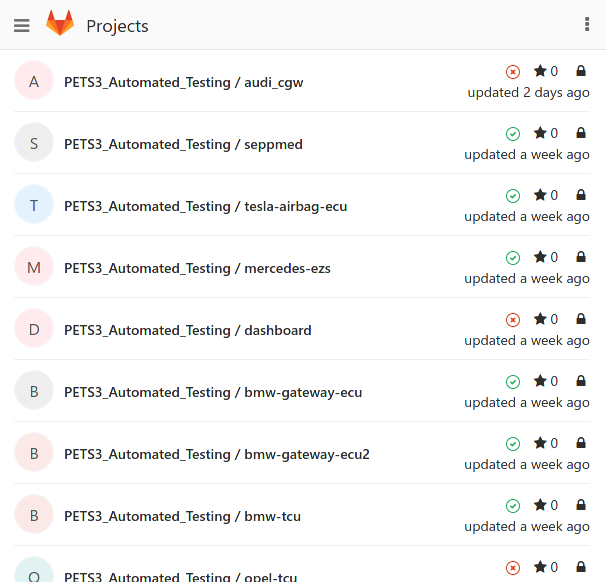
\includegraphics[width=0.7\textwidth]{gitlab-screenshot}
    \caption{Screenshot of the GitLab page from the LaS3 server.}
    \label{fig:gitlab-screenshot}
\end{figure}

Fifteen ECUs are available for testing on this server. However, three of them are from Opel and therefore only support GMLAN but not UDS. And two of them are identical, resulting in a total of eleven usable ECUs.

For each ECU a configuration file was created. Various work is done here, for example pulling and checking out the Scapy code from the currently working branch.

Then, the actual tests are executed that are implemented with the pytest framework. Here, a UDS scan can be started. At the same time, another process is started to record all CAN traffic that takes place during the execution of the tests (see \autoref{subsubsec:can-utils}).

Finally, the resulting files are uploaded to the GitLab server so that they can be downloaded via a browser program.

\section{Explaining the generated data of a scan}

In total, four files are stored after a scan, which will be explained in this section.

\begin{itemize}
    \item candump.log
    \item generic.log
    \item profiling.csv
    \item data.pkl
\end{itemize}

\subsection{Record communication between scanner and ECU}

The resulting 'candump.log' file recorded with the command shown in \autoref{lst:can-utils} (line 3) has a simple structure. Each line represents a CAN frame.

\begin{samepage}
\begin{minted}{text}
    (<timestamp>) <interface> <identifier>#<data>
    (1611779255.926425) can1 714#03225FB2CCCCCCCC
    (1611779255.929936) can1 77E#037F2231AAAAAAAA
    (1611779255.935338) can1 714#03225FB3CCCCCCCC
    (1611779255.940680) can1 77E#037F2231AAAAAAAA
\end{minted}
\end{samepage}

Unfortunately, these files contain a lot of information that is not only not needed, but also unwanted, as it leads to more difficult analysis because of higher storage and processing power usage. \autoref{fig:can-unwanted-information} shows the information that is not needed because it is ECU specific and does not add any value for the analysis.

%CAN unwanted information
\begin{figure}[H]
    \centering
    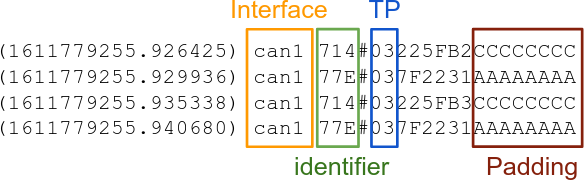
\includegraphics[width=0.7\textwidth]{can-unwanted-information}
    \caption{ECU specific information in candump.log.}
    \label{fig:can-unwanted-information}
\end{figure}

Consequently, an abstraction is desirable. The newly created format is called the generic format. It removes the interface, the padding, resolves the transport protocol information (ISO-TP) and replaces the identifier with representatives (s = Server, c = Client). Each line represents UDS data, instead of a lower layer CAN frame as in the candump logs. \autoref{fig:candump-generic-conversion} illustrates the input and output of a conversion.

%candump to generic conversion
\begin{figure}[htb]
    \centering
    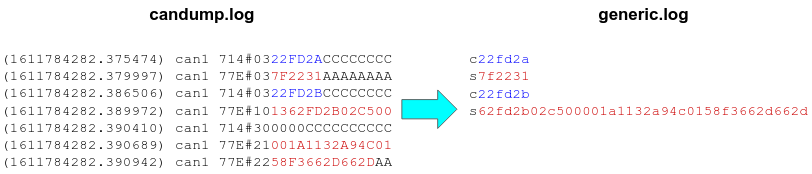
\includegraphics[width=1\textwidth]{candump-generic-conversion}
    \caption{candump.log to generic.log conversion.}
    \label{fig:candump-generic-conversion}
\end{figure}

This format proved to be very useful as it allows quick analysis by chaining common Linux programs.
For instance, counting the number of requests of a scan is a single command:
\begin{listing}[H]
\begin{minted}{bash}
        $ grep '^c.*' -c generic.log
        988844
\end{minted}
\caption{Example usage of the generic format.}
\label{lst:usage-generic}
\end{listing}

\subsection{Store service scan behavior of a scan}

For profiling, a file has been added as output to the UDS scanner, namely 'profiling.csv'. It contains which service scan ran under which state and when. It follows a fairly simple structure:

\begin{samepage}
    \begin{minted}{text}
        state     ,service  ,start            ,end
        ECU Reset ,ECU Reset,1611770228.135198,1611770228.658480
        [session1],CC       ,1611770228.661016,1611770231.236505
        ECU Reset ,ECU Reset,1611770231.236789,1611770231.754865
        [session1],DSC      ,1611770231.756320,1611770231.895722
    \end{minted}
\end{samepage}

The start and end timestamps are specified in Unix times.

Although an ECU Reset has no state, all occurrences of it are given the same named state for better visualization of the log later.

\subsection{Store the finished scanner object}

The 'data.pkl' file is the serialized UDS Scanner object after the scan and thus contains all the results, consisting of the responses for each request for each state of an ECU. This is helpful for debugging, analysis and also for simulation. 'pkl' stands for 'pickle', which is the name of the object serialization module of the Python standard library \cite{pickle}. 


\section{Profiling the UDS Scanner}

The Pareto principle indicates that small number of causes can be responsible for a large percentage of effects \cite{pareto}. This is also applicable to optimization problems. Usually only a few number of code lines cause the majority of the runtime. Optimizing them is far more effective than performing micro-optimizations as they naturally improve the performance to a greater extent. Moreover, micro-optimizations are usually even more difficult to accomplish.

\subsection{Visualizing UDS scans}

To profile the UDS Scanner, the 'profiling.csv' file is used. With its help Gantt charts are created which show the sequence and duration of the scanned services. This visualizes what parts of the UDS Scanner cause most of its runtime.

These charts have been created for each available ECU, with each color representing a state. For illustration, one is sufficient since each showed the same gist (see \autoref{fig:tesla-gantt})

\begin{figure}[H]
    \centering
    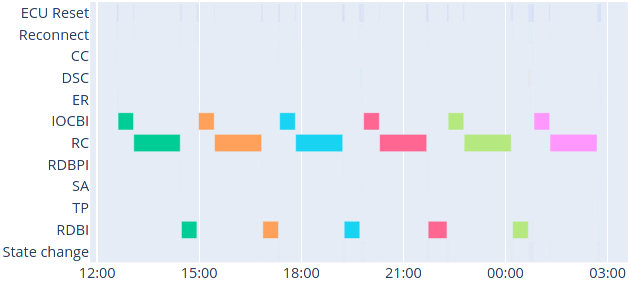
\includegraphics[width=0.9\textwidth]{tesla-gantt}
    \caption{Gantt chart of the Tesla-Airbag-ECU.}
    \label{fig:tesla-gantt}
\end{figure}


\subsection{Identifying the services causing the most runtime}

Although it seems that some services and events do not require any time, their time consumption is only so small that they are not or hardly visible in this scaled-down version of the diagram.

The main cause of runtime is the scan of the RC service. This was expected, since it requires the most requests.
In second place are the IOCBI and the RDBI service. They generate the same runtime, this was to be expected as well since they require the same number of requests. However, the IOCBI service is less frequently supported by ECUs than the RDBI service, resulting in a smaller runtime contribution when considering approach 3.

In summary, the RC and the RDBI service are the most critical runtime causes of the UDS scanner and therefore belong to the matters to be optimized.
